\documentclass[twoside,titlepage,11pt]{article}
%%\documentclass[titlepage,11pt]{article}

\usepackage{makeidx}
\usepackage{xtab}
\usepackage{amsmath, amssymb}

% Package to add Bibliography and Index to TOC
% but not the TOC itself :-)
\usepackage[nottoc]{tocbibind}

\usepackage{calc}

% Packages for adding figures
\usepackage{subfigure}
\usepackage{color}
\usepackage{graphicx}

% Needed for sideways
\usepackage{rotating}

% Packages used for output and source code listings
\usepackage{fancyvrb}
\usepackage{listings}

%\usepackage{fancyheadings}
\usepackage{fancyhdr}

% External references
\usepackage{xr}

% show margin lines for debugging
%\usepackage[showframe]{geometry}

%----- Define some colors
\definecolor{gray}{rgb}{0.5,0.5,0.5}

%----- Define the warning sign

\newcommand{\marginlabel}[1]
{\mbox{}\marginpar{\raggedleft\hspace{0pt}{\rule{0mm}{1mm}#1}}}

\newcommand{\warn}{%
%\marginlabel{\pstribox[shadow=false,fillstyle=solid,fillcolor=yellow,trimode=*U]{\footnotesize !}}%%
\marginlabel{
\includegraphics[scale=0.8]{warning}}%%
}

%----- Page formatting

\setlength{\paperwidth}{8.5in}
\setlength{\textwidth}{6.1in}
\setlength{\hoffset}{0.0in}
\setlength{\oddsidemargin}{0.2in}
\setlength{\evensidemargin}{0.2in}
\setlength{\marginparsep}{0.25in}
\setlength{\marginparwidth}{0.5in}

\setlength{\paperheight}{11.0in}
\setlength{\textheight}{9.0in}
\setlength{\voffset}{-0.25in}
\setlength{\topmargin}{0.0in}

%----- VERSIONS AND UCRL NUMBERS OF SUNDIALS CODES

\newcommand{\sunrelease}{v6.1.1}

\newcommand{\cvrelease}{v6.1.1}
\newcommand{\cvucrlug}{UCRL-SM-208108}
\newcommand{\cvucrlex}{UCRL-SM-208110}

\newcommand{\cvsrelease}{v6.1.1}
\newcommand{\cvsucrlug}{UCRL-SM-208111}
\newcommand{\cvsucrlex}{UCRL-SM-208115}

\newcommand{\idarelease}{v6.1.1}
\newcommand{\idaucrlug}{UCRL-SM-208112}
\newcommand{\idaucrlex}{UCRL-SM-208113}

\newcommand{\idasrelease}{v5.1.1}
\newcommand{\idasucrlug}{UCRL-SM-234051}
\newcommand{\idasucrlex}{LLNL-TR-437091}

\newcommand{\kinrelease}{v6.1.1}
\newcommand{\kinucrlug}{UCRL-SM-208116}
\newcommand{\kinucrlex}{UCRL-SM-208114}

\newcommand{\arkrelease}{v5.1.1}
\newcommand{\arkucrlug}{LLNL-SM-668082}
\newcommand{\arkucrlex}{????-??-??????}

%----- SUNDIALS MODULES
\newcommand{\sundials}{{\normalfont\scshape sundials}}
\newcommand{\shared}{{\normalfont\scshape shared}}
%----- Vectors:
\newcommand{\nvector}{{\normalfont\scshape nvector}}
\newcommand{\fnvector}{{\normalfont\scshape fnvector}}
\newcommand{\nvecs}{{\normalfont\scshape nvector\_serial}}
\newcommand{\nvecp}{{\normalfont\scshape nvector\_parallel}}
\newcommand{\nvecopenmp}{{\normalfont\scshape nvector\_openmp}}
\newcommand{\nvecopenmpdev}{{\normalfont\scshape nvector\_openmpdev}}
\newcommand{\nvecpthreads}{{\normalfont\scshape nvector\_pthreads}}
\newcommand{\nvecph}{{\normalfont\scshape nvector\_parhyp}}
\newcommand{\nvecpetsc}{{\normalfont\scshape nvector\_petsc}}
\newcommand{\nveccuda}{{\normalfont\scshape nvector\_cuda}}
\newcommand{\nvechip}{{\normalfont\scshape nvector\_hip}}
\newcommand{\nvecraja}{{\normalfont\scshape nvector\_raja}}
\newcommand{\nvecsycl}{{\normalfont\scshape nvector\_sycl}}
\newcommand{\nvectrilinos}{{\normalfont\scshape nvector\_trilinos}}
\newcommand{\nvecwrap}{{\normalfont\scshape nvector\_senswrapper}}
\newcommand{\nvecmanyvector}{{\normalfont\scshape nvector\_manyvector}}
\newcommand{\nvecmpimanyvector}{{\normalfont\scshape nvector\_mpimanyvector}}
\newcommand{\nvecmpiplusx}{{\normalfont\scshape nvector\_mpiplusx}}
%----- Matrices:
\newcommand{\sunmatrix}{{\normalfont\scshape sunmatrix}}
\newcommand{\fsunmatrix}{{\normalfont\scshape fsunmatrix}}
\newcommand{\sunmatband}{{\normalfont\scshape sunmatrix\_band}}
\newcommand{\sunmatdense}{{\normalfont\scshape sunmatrix\_dense}}
\newcommand{\sunmatsparse}{{\normalfont\scshape sunmatrix\_sparse}}
\newcommand{\sunmatcusparse}{{\normalfont\scshape sunmatrix\_cusparse}}
\newcommand{\sunmatslunrloc}{{\normalfont\scshape sunmatrix\_slunrloc}}
%----- Linear Solvers:
\newcommand{\sunlinsol}{{\normalfont\scshape sunlinsol}}
\newcommand{\fsunlinsol}{{\normalfont\scshape fsunlinsol}}
\newcommand{\sunlinsolband}{{\normalfont\scshape sunlinsol\_band}}
\newcommand{\sunlinsoldense}{{\normalfont\scshape sunlinsol\_dense}}
\newcommand{\sunlinsollapband}{{\normalfont\scshape sunlinsol\_lapackband}}
\newcommand{\sunlinsollapdense}{{\normalfont\scshape sunlinsol\_lapackdense}}
\newcommand{\sunlinsolklu}{{\normalfont\scshape sunlinsol\_klu}}
\newcommand{\sunlinsolsludist}{{\normalfont\scshape sunlinsol\_superludist}}
\newcommand{\sunlinsolslumt}{{\normalfont\scshape sunlinsol\_superlumt}}
\newcommand{\sunlinsolcuspbqr}{{\normalfont\scshape sunlinsol\_cusolversp\_batchqr}}
\newcommand{\sunlinsolspgmr}{{\normalfont\scshape sunlinsol\_spgmr}}
\newcommand{\sunlinsolspfgmr}{{\normalfont\scshape sunlinsol\_spfgmr}}
\newcommand{\sunlinsolspbcgs}{{\normalfont\scshape sunlinsol\_spbcgs}}
\newcommand{\sunlinsolsptfqmr}{{\normalfont\scshape sunlinsol\_sptfqmr}}
\newcommand{\sunlinsolpcg}{{\normalfont\scshape sunlinsol\_pcg}}
\newcommand{\sunlinsolcusparse}{{\normalfont\scshape sunlinsol\_cusparse}}
%----- Nonlinear Solvers:
\newcommand{\sunnonlinsol}{{\normalfont\scshape sunnonlinsol}}
\newcommand{\fsunnonlinsol}{{\normalfont\scshape fsunnonlinsol}}
\newcommand{\sunnonlinsolnewton}{{\normalfont\scshape sunnonlinsol\_newton}}
\newcommand{\sunnonlinsolfixedpoint}{{\normalfont\scshape sunnonlinsol\_fixedpoint}}
\newcommand{\sunnonlinsolpetsc}{{\normalfont\scshape sunnonlinsol\_petscsnes}}
%----- SUNMemory:
\newcommand{\sunmemory}{{\normalfont\scshape sunmemory}}
%----- Packages:
\newcommand{\cvode}{{\normalfont\scshape cvode}}
\newcommand{\pvode}{{\normalfont\scshape pvode}}
\newcommand{\cvodes}{{\normalfont\scshape cvodes}}
\newcommand{\arkode}{{\normalfont\scshape arkode}}
\newcommand{\ida}{{\normalfont\scshape ida}}
\newcommand{\idas}{{\normalfont\scshape idas}}
\newcommand{\kinsol}{{\normalfont\scshape kinsol}}
\newcommand{\sundialsTB}{{\normalfont\scshape sundialsTB}}

%----- OTHER PACKAGES
\newcommand{\vode}{{\normalfont\scshape vode}}
\newcommand{\vodpk}{{\normalfont\scshape vodpk}}
\newcommand{\lsode}{{\normalfont\scshape lsode}}
\newcommand{\daspk}{{\normalfont\scshape daspk}}
\newcommand{\daspkadjoint}{{\normalfont\scshape daspkadjoint}}
\newcommand{\hypre}{\textsl{hypre}}
\newcommand{\openmp}{{\normalfont OpenMP}}
\newcommand{\petsc}{{\normalfont\scshape pets}c}
\newcommand{\cuda}{{\normalfont\scshape cuda}}
\newcommand{\hip}{{\normalfont\scshape hip}}
\newcommand{\raja}{{\normalfont\scshape raja}}
\newcommand{\sycl}{{\normalfont\scshape sycl}}
\newcommand{\superludist}{SuperLU\_DIST}
\newcommand{\trilinos}{Trilinos}
\newcommand{\tpetra}{Tpetra}

%----- CVODE and CVODES COMPONENTS
\newcommand{\cvnls}{{\normalfont\scshape cvnls}}
\newcommand{\cvdls}{{\normalfont\scshape cvdls}}
\newcommand{\cvsls}{{\normalfont\scshape cvsls}}
\newcommand{\cvcls}{{\normalfont\scshape cvcls}}
\newcommand{\cvls}{{\normalfont\scshape cvls}}
\newcommand{\cvdense}{{\normalfont\scshape cvdense}}
\newcommand{\cvsparse}{{\normalfont\scshape cvsparse}}
\newcommand{\cvband}{{\normalfont\scshape cvband}}
\newcommand{\cvdiag}{{\normalfont\scshape cvdiag}}
\newcommand{\cvspils}{{\normalfont\scshape cvspils}}
\newcommand{\cvspgmr}{{\normalfont\scshape cvspgmr}}
\newcommand{\cvspbcg}{{\normalfont\scshape cvspbcg}}
\newcommand{\cvsptfqmr}{{\normalfont\scshape cvsptfqmr}}
\newcommand{\cvklu}{{\normalfont\scshape cvklu}}
\newcommand{\cvsuperlumt}{{\normalfont\scshape cvsuperlumt}}
\newcommand{\cvbandpre}{{\normalfont\scshape cvbandpre}}
\newcommand{\cvbbdpre}{{\normalfont\scshape cvbbdpre}}
\newcommand{\cvodea}{{\normalfont\scshape cvodea}}
\newcommand{\fcvode}{{\normalfont\scshape fcvode}}
\newcommand{\fcvbp}{{\normalfont\scshape fcvbp}}
\newcommand{\fcvbbd}{{\normalfont\scshape fcvbbd}}
\newcommand{\fcvroot}{{\normalfont\scshape fcvroot}}
\newcommand{\stald}{{\normalfont\scshape stald}}

%----- KINSOL COMPONENTS
\newcommand{\kinspils}{{\normalfont\scshape kinspils}}
\newcommand{\kinspgmr}{{\normalfont\scshape kinspgmr}}
\newcommand{\kinspfgmr}{{\normalfont\scshape kinspfgmr}}
\newcommand{\kinspbcg}{{\normalfont\scshape kinspbcg}}
\newcommand{\kinsptfqmr}{{\normalfont\scshape kinsptfqmr}}
\newcommand{\kinbbdpre}{{\normalfont\scshape kinbbdpre}}
\newcommand{\kindls}{{\normalfont\scshape kindls}}
\newcommand{\kincls}{{\normalfont\scshape kincls}}
\newcommand{\kinsls}{{\normalfont\scshape kinsls}}
\newcommand{\kinls}{{\normalfont\scshape kinls}}
\newcommand{\kindense}{{\normalfont\scshape kindense}}
\newcommand{\kinband}{{\normalfont\scshape kinband}}
\newcommand{\kinsparse}{{\normalfont\scshape kinsparse}}
\newcommand{\kinklu}{{\normalfont\scshape kinklu}}
\newcommand{\kinsuperlumt}{{\normalfont\scshape kinsuperlumt}}
\newcommand{\fkinbbd}{{\normalfont\scshape fkinbbd}}
\newcommand{\fkindense}{{\normalfont\scshape fkindense}}
\newcommand{\fkinband}{{\normalfont\scshape fkinband}}
\newcommand{\fkinsol}{{\normalfont\scshape fkinsol}}

%----- IDA and IDAS COMPONENTS
\newcommand{\idanls}{{\normalfont\scshape idanls}}
\newcommand{\idadls}{{\normalfont\scshape idadls}}
\newcommand{\idacls}{{\normalfont\scshape idacls}}
\newcommand{\idasls}{{\normalfont\scshape idasls}}
\newcommand{\idals}{{\normalfont\scshape idals}}
\newcommand{\idadense}{{\normalfont\scshape idadense}}
\newcommand{\idasparse}{{\normalfont\scshape idasparse}}
\newcommand{\idaband}{{\normalfont\scshape idaband}}
\newcommand{\idaklu}{{\normalfont\scshape idaklu}}
\newcommand{\idasuperlumt}{{\normalfont\scshape idasuperlumt}}
\newcommand{\idaspils}{{\normalfont\scshape idaspils}}
\newcommand{\idaspgmr}{{\normalfont\scshape idaspgmr}}
\newcommand{\idaspbcg}{{\normalfont\scshape idaspbcg}}
\newcommand{\idasptfqmr}{{\normalfont\scshape idasptfqmr}}
\newcommand{\idabbdpre}{{\normalfont\scshape idabbdpre}}
\newcommand{\idaa}{{\normalfont\scshape idaa}}
\newcommand{\fida}{{\normalfont\scshape fida}}
\newcommand{\fidaband}{{\normalfont\scshape fidaband}}
\newcommand{\fidadense}{{\normalfont\scshape fidadense}}
\newcommand{\fidabbd}{{\normalfont\scshape fidabbd}}
\newcommand{\fidaroot}{{\normalfont\scshape fidaroot}}

%----- SHARED COMPONENTS
\newcommand{\sundialsmath}{{\normalfont\scshape sundialsmath}}
\newcommand{\diag}{{\normalfont\scshape diag}}
\newcommand{\dense}{{\normalfont\scshape dense}}
\newcommand{\band}{{\normalfont\scshape band}}
\newcommand{\pcg}{{\normalfont\scshape pcg}}
\newcommand{\sls}{{\normalfont\scshape sls}}
\newcommand{\sparse}{{\normalfont\scshape sparse}}
\newcommand{\spgmr}{{\normalfont\scshape spgmr}}
\newcommand{\spfgmr}{{\normalfont\scshape spfgmr}}
\newcommand{\spbcg}{{\normalfont\scshape spbcgs}}
\newcommand{\spbcgs}{{\normalfont\scshape spbcgs}}
\newcommand{\sptfqmr}{{\normalfont\scshape sptfqmr}}
\newcommand{\klu}{{\normalfont\scshape klu}}
\newcommand{\superlumt}{{\normalfont\scshape superlumt}}

%----- OS
\newcommand{\linux}{{\sc LINUX}}
\newcommand{\unix}{{\sc UNIX}}
\newcommand{\mpi}{{\sc MPI}}

%----- C and Fortran languages
\newcommand{\CC}{{\sc C}}
\newcommand{\CPP}{{\sc C}\raisebox{0.2em}{\tiny ++}}
\newcommand{\F}{{\sc Fortran}}

%------ Serial, OpenMP, Pthreads, Parallel, or ParHyp
\newcommand{\s}{[{\bf S}]}
\newcommand{\omp}{[{\bf O}]}
\newcommand{\pt}{[{\bf T}]}
\newcommand{\p}{[{\bf P}]}
\newcommand{\h}{[{\bf H}]}

%------ Appendix in text
\newcommand{\A}{App. }

%------ Index entries

\newcommand{\ID}[1]{{\tt #1}{\index{#1@\texttt{#1}}}}
%\newcommand{\ID}[1]{{\tt #1}{\index{#1@\texttt{#1}|textbf}}}
% NOTE: the above version confuses hyperref...
\newcommand{\Id}[1]{{\tt #1}{\index{#1@\texttt{#1}}}}
\newcommand{\id}[1]{{\tt #1}}

%%----- Shortcuts for math formulas
\newcommand{\mb}[1]{{\mbox{\scriptsize #1}}}

\newcommand{\dfdy}{\frac{\partial f}{\partial y}}
\newcommand{\dfdyI}{\partial f / \partial y}
\newcommand{\dfdpi}{\frac{\partial f}{\partial p_i}}
\newcommand{\dfdpiI}{\partial f / \partial p_i}

\newcommand{\dFdy}{\frac{\partial F}{\partial y}}
\newcommand{\dFdyI}{\partial F / \partial y}
\newcommand{\dFdyp}{\frac{\partial F}{\partial \dot y}}
\newcommand{\dFdypI}{\partial F / \partial \dot y}
\newcommand{\dFdpi}{\frac{\partial F}{\partial p_i}}
\newcommand{\dFdpiI}{\partial F / \partial p_i}

\newcommand{\rhomax}{\rho_{\max}}

\newcommand{\cm}{$\checkmark$}

\newcommand{\newlinefill}[1]{\newline\phantom{#1}}

%%------ Specify depths for section numbering and TOC

\setcounter{tocdepth}{1}
\setcounter{secnumdepth}{3}

%%-------

\newcommand{\includeCode}[1]
{
  \VerbatimInput[numbers=left,fontsize=\small]{#1}
}

\newcommand{\includeOutput}[2]
{
  \vspace{0.1in}
  \VerbatimInput[frame=single,
                 framesep=0.1in,
                 label={\tt #1} sample output,
                 fontsize=\footnotesize]{#2}
}

%%-------

\newcommand{\ugref}[1]{\S\ref{#1}}

%%-------

\newcommand{\clearemptydoublepage}{\newpage{\pagestyle{empty}\cleardoublepage}}

%%-------

\newcommand{\disclaimer}{%
\thispagestyle{empty}% no number of this page
\vglue5\baselineskip
\begin{center}
{\bf DISCLAIMER}
\end{center}
\noindent
This document was prepared as an account of work sponsored by an agency of
the United States government. Neither the United States government nor
Lawrence Livermore National Security, LLC, nor any of their employees makes
any warranty, expressed or implied, or assumes any legal liability or responsibility
for the accuracy, completeness, or usefulness of any information, apparatus, product,
or process disclosed, or represents that its use would not infringe privately owned rights.
Reference herein to any specific commercial product, process, or service by trade name,
trademark, manufacturer, or otherwise does not necessarily constitute or imply its endorsement,
recommendation, or favoring by the United States government or Lawrence Livermore National
Security, LLC. The views and opinions of authors expressed herein do not necessarily state
or reflect those of the United States government or Lawrence Livermore National Security, LLC,
and shall not be used for advertising or product endorsement purposes.

\vskip2\baselineskip
\noindent This work was performed under the auspices of the U.S. Department of Energy by Lawrence
Livermore National Laboratory under Contract DE-AC52-07NA27344.
\vfill
\begin{center}
Approved for public release; further dissemination unlimited
\end{center}
\clearpage
}

%%-------

\newcommand{\contributors}{%
\thispagestyle{empty}% no number of this page
\vglue5\baselineskip
\begin{center}
{\bf CONTRIBUTORS}
\end{center}
\noindent
The SUNDIALS library has been developed over many years by a number of
contributors. The current SUNDIALS team consists of Cody J. Balos,
David J. Gardner, Alan C. Hindmarsh, Daniel R. Reynolds, and
Carol S. Woodward. We thank Radu Serban for significant and critical past
contributions.\\
\\
\noindent
Other contributors to SUNDIALS include: James Almgren-Bell, Lawrence E. Banks,
Peter N. Brown, George Byrne, Rujeko Chinomona, Scott D. Cohen, Aaron Collier,
Keith E. Grant, Steven L. Lee, Shelby L. Lockhart, John Loffeld, Daniel McGreer,
Slaven Peles, Cosmin Petra, H. Hunter Schwartz, Jean M. Sexton,
Dan Shumaker, Steve G. Smith, Allan G. Taylor, Hilari C. Tiedeman, Chris White,
Ting Yan, and Ulrike M. Yang.
\clearpage
}

%%--------------------------------

\newcommand{\frontug}
{

  %% Start roman numbering
  \pagenumbering{roman}

  %% Title page
  \maketitle
  \disclaimer
  \contributors
  \clearemptydoublepage

  %% Contents, tables, and figures
  \tableofcontents
  \clearemptydoublepage
  \listoftables
  \clearemptydoublepage
  \listoffigures
  \clearemptydoublepage

  %% Start arabic numbering
  \pagenumbering{arabic}

  %% Define page style for the body of the document
  \lhead[\fancyplain{}{\bfseries\thepage}]%
        {\fancyplain{}{\bfseries\rightmark}}
  \rhead[\fancyplain{}{\bfseries\leftmark}]%
        {\fancyplain{}{\bfseries\thepage}}
  \cfoot{}
  \pagestyle{fancyplain}


  %% Some settings for code listings
  \lstset{
    language=C, fancyvrb=true,
    basicstyle=\footnotesize\ttfamily,
    commentstyle=\color{MidnightBlue},
    keywordstyle=\color{BrickRed},
    stringstyle=\color{OliveGreen},
    numbers=left, numberstyle=\tiny, numbersep=15pt}

}

%%--------------------------------
\newcommand{\frontex}
{

  \pagestyle{empty}
  \maketitle
  \disclaimer
  \contributors
  \clearemptydoublepage

  % Contents
  \tableofcontents

  %% Start arabic numbering
  \clearemptydoublepage
  %%\clearpage
  \pagestyle{plain}\pagenumbering{arabic}

  %% Some settings for code listings
  \lstset{
    fancyvrb=true,
    basicstyle=\footnotesize\ttfamily,
    commentstyle=\color{MidnightBlue},
    keywordstyle=\color{BrickRed},
    stringstyle=\color{OliveGreen},
    numbers=left, numberstyle=\tiny, numbersep=15pt}

}

%%----------------------------------
%% List of configure options
%%---------------------------------
\newenvironment{config}
{\begin{list}{}{
      \setlength{\leftmargin}{2em}
      \setlength{\rightmargin}{0em}
      \setlength{\topsep}{0.05in}
      \setlength{\itemindent}{-2em}
      \setlength{\itemsep}{0.05in}}}
  {\end{list}}
%%---------------------------------
%% Steps used in skeleton programs
%%---------------------------------
\newcounter{Stepsctr}
\newenvironment{Steps}
{\stepcounter{Stepsctr}
  \begin{list}{\arabic{Stepsctr}. }{
      \usecounter{Stepsctr}
      \setlength{\parsep}{0.5em}
      \setlength{\labelsep}{0em}
      \settowidth{\labelwidth}{99. }
      \setlength{\leftmargin}{\labelwidth+\labelsep}}}
  {\end{list}}
%%-----------------------------------------------------
%% Underlying list environemnt for function definitions
%%-----------------------------------------------------
\newenvironment{Ventry}[1][\quad]
{\begin{list}{}{
      \setlength{\rightmargin}{0em}
      \setlength{\topsep}{0.05in}
      \setlength{\itemsep}{0em}
      \setlength{\itemindent}{0em}
      \setlength{\labelsep}{0.5em}
      \renewcommand{\makelabel}[1]{##1\hfill}
      \settowidth{\labelwidth}{#1}
      \setlength{\leftmargin}{\labelwidth+\labelsep}}}
  {\end{list}}
%%----------------------------------
%% List of function arguments
%%---------------------------------
\newenvironment{args}[1][\quad]
{\begin{list}{}{
      \setlength{\rightmargin}{0em}
      \setlength{\topsep}{0em}
      \setlength{\itemsep}{0em}
      \setlength{\itemindent}{0em}
      \setlength{\labelsep}{0.5em}
      \renewcommand{\makelabel}[1]{\id{##1}\hfill}
      \settowidth{\labelwidth}{\id{#1}}
      \setlength{\leftmargin}{\labelwidth+\labelsep}}}
  {\end{list}}
%%---------------------------------
%% User-callable function
%%---------------------------------
\newcommand{\ucfunction}[6]{
  \noindent\paragraph{\fbox{\id{#1}}}
  \begin{Ventry}[Return value]
  \item[Call]{\id{#2}}
  \item[Description]{#3}
  \addArgs{#4}
  \addRetval{#5}
  \addNotes{#6}
  \end{Ventry}
}
%%----------------------------------------------
%% User-callable function with a deprecated name
%%----------------------------------------------
\newcommand{\ucfunctiond}[7]{
  \noindent\paragraph{\fbox{\id{#1}}}
  \begin{Ventry}[Deprecated Name]
  \item[Call]{\id{#2}}
  \item[Description]{#3}
  \addArgs{#4}
  \addRetval{#5}
  \addNotes{#6}
  \addDepName{#7}
  \end{Ventry}
}
%%-----------------------------------------------------
%% User-callable function with a Fortran 2003 interface
%%-----------------------------------------------------
\newcommand{\ucfunctionf}[6]{
  \noindent\paragraph{\fbox{\id{#1}}}
  \begin{Ventry}[Return value]
  \item[Call]{\id{\begin{tabular}[t]{@{}r@{}l@{}}#2\end{tabular}}}
  \item[Description]{#3}
  \addArgs{#4}
  \addRetval{#5}
  \addNotes{#6}
  \item[F2003 Name]{\id{F#1}}
  \end{Ventry}
}
%%-----------------------------------------------------
%% User-callable function with a Fortran 2003 interface
%% and an additional entry on how to call the F2003
%% function.
%%-----------------------------------------------------
\newcommand{\ucfunctionfl}[7]{
  \noindent\paragraph{\fbox{\id{#1}}}
  \begin{Ventry}[Return value]
  \item[Call]{\id{#2}}
  \item[Description]{#3}
  \addArgs{#4}
  \addRetval{#5}
  \addNotes{#6}
  \item[F2003 Name]{\id{F#1}}
  \item[F2003 Call]{\id{#7}}
  \end{Ventry}
}
%%-----------------------------------------------------
%% User-callable function with a deprecated name and
%% a Fortran 2003 interface
%%-----------------------------------------------------
\newcommand{\ucfunctiondf}[7]{
  \noindent\paragraph{\fbox{\id{#1}}}
  \begin{Ventry}[Deprecated Name]
  \item[Call]{\id{#2}}
  \item[Description]{#3}
  \addArgs{#4}
  \addRetval{#5}
  \addNotes{#6}
  \addDepName{#7}
  \item[F2003 Name]{\id{F#1}}
  \end{Ventry}
}
%%--------------------------------------------
%% macro for generic SUNDIALS module functions
%%--------------------------------------------
\newcommand{\sunmodfun}[3]{
  \noindent\paragraph{\fbox{\ID{#1}}}
  \begin{Ventry}[F2003 Name]
  \item[Prototype]{\id{#3}}
  \item[Description]{#2}
  \end{Ventry}
}
%%-------------------------------------------------------
%% macro for generic overloaded SUNDIALS module functions
%%-------------------------------------------------------
\newcommand{\sunmodfuns}[6]{
  \noindent\paragraph{\fbox{\ID{#1}}}
  \begin{Ventry}[F2003 Name]
  \item[\textit{Single-node usage}]{}
  \item[Prototype]{\id{#4}}
  \item[Description]{#2#3}
  \item[\textit{Distributed-memory parallel usage}]{}
  \item[Prototype]{\id{#6}}
  \item[Description]{#2#5}
  \end{Ventry}
}
%%--------------------------------------------------------------------------
%% macro for generic SUNDIALS module functions with a Fortran 2003 interface
%%--------------------------------------------------------------------------
\newcommand{\sunmodfunf}[3]{
  \noindent\paragraph{\fbox{\ID{#1}}}
  \begin{Ventry}[F2003 Name]
  \item[Prototype]{\id{#3}}
  \item[Description]{#2}
  \item[F2003 Name]{This function is callable as \id{F#1} when using the Fortran
  2003 interface module.}
  \end{Ventry}
}
%%---------------------------------
%% User-supplied function
%%---------------------------------
\newcommand{\usfunction}[6]{
  \noindent\paragraph{\fbox{\id{#1}}}
  \begin{Ventry}[Return value]
  \item[Definition]{\id{\begin{tabular}[t]{@{}r@{}l@{}}#2\end{tabular}}}
  \item[Purpose]{#3}
  \item[Arguments]{#4}
  \item[Return value]{#5}
  \addNotes{#6}
  \end{Ventry}
}
%%---------------------------------
\makeatletter
\long\def\addArgs#1{\def\@tempa{#1}\ifx\@tempa\empty\item[Arguments]{None}\else\item[Arguments]{#1}\fi}
\makeatother
%%---------------------------------
\makeatletter
\long\def\addRetval#1{\def\@tempa{#1}\ifx\@tempa\empty\item[Return value]{None}\else\item[Return value]{#1}\fi}
\makeatother
%%---------------------------------
\makeatletter
\long\def\addNotes#1{\def\@tempa{#1}\ifx\@tempa\empty\else\item[Notes]{#1}\fi}
\makeatother
%%---------------------------------
\makeatletter
\long\def\addDepName#1{\def\@tempa{#1}\ifx\@tempa\empty\item[Deprecated
  Name]{None}\else\item[Deprecated Name]{For backward compatibility, the wrapper
  function \id{#1} with idential input and output arguments is also
  provided.}\fi}
\makeatother


%%---------------------------------
%% Finally, use hyperref package to include links in the PDF
%% Note that since hyperref redefines a bunch of LaTeX commands,
%% to give it a fighting chance, it MUST be included last.

\usepackage[
% letterpaper=true,
% dvips,
% ps2pdf,
hyperindex=true,
linktocpage=true,
colorlinks=true,
linkcolor=blue,
citecolor=blue,
bookmarks=true]
{hyperref}


\externaldocument{cvs_install}
\externaldocument{cvs_math}
\externaldocument{cvs_sim}
\externaldocument{cvs_fwd}
\externaldocument{cvs_adj}
\externaldocument{cvs_nvec}
\externaldocument{cvs_linsolv}


\newcommand{\cvsucrl}{UCRL-SM-208115}
\newcommand{\cvsdate}{April 2005}
\newcommand{\cvsrelease}{v2.2.0}

\renewcommand{\thefootnote}{\fnsymbol{footnote}}

\title{Example Programs for {\cvodes} \\ \cvsrelease}
\author{
  Alan C. Hindmarsh and Radu Serban\\
  {\em Center for Applied Scientific Computing} \\
  {\em Lawrence Livermore National Laboratory}
}
\date{\cvsdate \vfill \cvsucrl}

\begin{document}

%Create the LLNL Cover Page
%\makeLLNLCover{\cvsucrl}%                      UCRL number
%{Example Programs for CVODES {\cvsrelease}}%   Title on cover page
%{Alan C. Hindmarsh and Radu Serban}%           Authors
%{\cvsdate}%                                    Date
%{0in}{0in}

\frontex

%===============================================================
%===============================================================================
\section{Introduction}\label{s:ex_intro}
%===============================================================================

This report is intended to serve as a companion document to the User
Documentation of {\cvodes} \cite{cvodes2.1.0_ug}.  It provides details, with
listings, on the example programs supplied with the {\cvodes} distribution
package.

The {\cvode} distribution contains examples of the following types: 
serial and parallel examples for IVP integration, 
serial and parallel examples for forward sensitivity analysis, and 
serial and parallel examples for adjoint sensitivity analysis.
These examples, summarized below, are shortly described next.

\newlength{\colone}
\settowidth{\colone}{em*3}
%\newlength{\coltwo}
%\setlength{\coltwo}{(\textwidth-\colone-0.5in)/2}
\begin{center}
%  \begin{tabular}{|p{\colone}|p{\coltwo}|p{\coltwo}|} \hline
  \begin{tabular}{|p{\colone}|l|l|} \hline
    & Serial examples & Parallel examples \\ \hline
    IVP & 
    \id{cvbx} \id{cvdx} \id{cvdemd} \id{cvkx} \id{cvkxb} \id{cvdemk} &
    \id{pvkx} \id{pvkxb} \id{pvfnx} \\ \hline
    FSA &  
    \id{cvfdx} \id{cvfkx} \id{cvfnx}  & 
    \id{pvfnx} \id{pvfkx}\\ \hline
    ASA & 
    \id{cvabx} \id{cvadx} \id{cvakx} \id{cvakxb} & 
    \id{pvanx} \id{pvakx} \\ \hline
  \end{tabular}
\end{center}

\vspace{0.2in}
\noindent Supplied in the \id{sundials/cvodes/examples\_ser} directory are the
following thirteen serial examples (using the {\nvecs} module):

%%
%%--------------------------------------
%%
\begin{itemize}

\item \id{cvdx}
  solves a chemical kinetics problem consisting of three rate equations.

  This program solves the problem with the BDF method and Newton          
  iteration, with the {\cvdense} linear solver and a user-supplied    
  Jacobian routine.  It also uses the rootfinding feature of {\cvodes}.

\item \id{cvbx}
  solves the semi-discrete form of an advection-diffusion equation in 2-D. 

  This program solves the problem with the BDF method and Newton          
  iteration, with the {\cvband} linear solver and a user-supplied     
  Jacobian routine.

\item \id{cvkx}
  solves the semi-discrete form of a two-species diurnal kinetics
  advection-diffusion PDE system in 2-D.

  The problem is solved with the BDF/GMRES method (i.e.    
  using the {\cvspgmr} linear solver) and the block-diagonal part of the  
  Newton matrix as a left preconditioner. A copy of the block-diagonal 
  part of the Jacobian is saved and conditionally reused within the    
  preconditioner setup routine.

\item \id{cvkxb}
  solves the same problem as \id{cvkx}, with the BDF/GMRES method 
  and a banded preconditioner, generated by difference quotients, 
  using the module {\cvbandpre}.

  The problem is solved twice - with preconditioning on the left,
  then on the right.

\item \id{cvdemd}
  is a demonstration program for {\cvodes} with direct linear solvers.

  Two separate problems are solved using both the Adams and BDF linear
  multistep methods in combination with functional and Newton
  iterations. 

  The first problem is the Van der Pol oscillator for which 
  the Newton iteration cases use the following types of Jacobian approximations:
  (1) dense (user-supplied), (2) dense (difference quotient approximation), 
  (3) diagonal approximation. The second problem is a linear ODE with a
  banded lower triangular matrix derived from a 2-D advection PDE. In this
  case, the Newton iteration cases use the following types of Jacobian
  approximation: (1) banded (user-supplied), (2) banded (difference quotient
  approximation), (3) diagonal approximation.

\item \id{cvdemk}
  is a demonstration program for {\cvodes} with the Krylov linear solver.

  This program solves a stiff ODE system that arises from a system     
  of partial differential equations.  The PDE system is a six-species
  food web population model, with predator-prey interaction and diffusion 
  on the unit square in two dimensions.

  The ODE system is solved using Newton iteration and the      
  {\cvspgmr} linear solver (scaled preconditioned GMRES).

  The preconditioner matrix used is the product of two matrices:         
  (1) a matrix, only implicitly defined, based on a fixed number of     
  Gauss-Seidel iterations using the diffusion terms only; and               
  (2) a block-diagonal matrix based on the partial derivatives of the   
  interaction terms only, using block-grouping.                          

  Four different runs are made for this problem.                        
  The product preconditoner is applied on the left and on the right.    
  In each case, both the modified and classical Gram-Schmidt options    
  are tested.

\item \id{cvfdx}
  solves a chemical kinetics problem consisting of three rate equations.

  {\cvodes} computes both its solution and solution sensitivities with respect
  to the three reaction rate constants appearing in the model. 
  This program solves the problem with the BDF method, Newton          
  iteration with the {\cvdense} linear solver, and a user-supplied    
  Jacobian routine.

\item \id{cvfkx}
  solves the semi-discrete form of a two-species diurnal kinetics
  advection-diffusion PDE system in 2-D space.

  {\cvodes} computes both its solution and solution sensitivities with respect
  to two parameters affecting the kinetic rate terms.
  The problem is solved with the BDF/GMRES method (i.e. using the {\cvspgmr}
  linear solver) and the block-diagonal part of the  
  Newton matrix as a left preconditioner.

\item \id{cvfnx}
  solves the semi-discrete form of an advection-diffusion equation in 1-D.

  {\cvodes} computes both its solution and solution sensitivities with respect
  to the advection and diffusion coefficients.
  This program solves the problem with the option for nonstiff systems,
  i.e. Adams method and functional iteration.

\item \id{cvabx}
  solves the semi-discrete form of an advection-diffusion equation in 2-D.

  The adjoint capability of {\cvodes} is used to compute gradients
  of the average (over both time and space) of the solution with respect to
  the initial conditions.
  This program solves both the forward and backward problems with the BDF method, 
  Newton iteration with the {\cvband} linear solver, and user-supplied     
  Jacobian routines.

\item \id{cvadx}
  solves a chemical kinetics problem consisting of three rate equations.
  
  The adjoint capability of {\cvodes} is used to compute gradients
  of a functional of the solution with respect to the three
  reaction rate constants appearing in the model.
  This program solves both the forward and backward problems with the BDF method, 
  Newton iteration with the {\cvdense} linear solver, and user-supplied    
  Jacobian routines.

\item \id{cvakx}
  solves a stiff ODE system that arises from a system     
  of partial differential equations.  The PDE system is a six-species
  food web population model, with predator-prey interaction and diffusion 
  on the unit square in two dimensions.

  The adjoint capability of {\cvodes} is used to compute gradients
  of the average (over both time and space) of the concentration of a selected species
  with respect to the initial conditions of all six species.
  Both the forward and backward problems are solved with the BDF/GMRES method 
  (i.e. using the {\cvspgmr} linear solver) and the block-diagonal part of the  
  Newton matrix as a left preconditioner.

\item \id{cvakxb}
  solves the same problem as \id{cvakx}, but computes gradients
  of the average over space at the final time of the concentration of a selected species
  with respect to the initial conditions of all six species.

\end{itemize}
%%
%%--------------------------------------
%%

\vspace{0.2in}
\noindent Supplied in the \id{sundials/cvode/examples\_par} directory are
the following six parallel examples (using the {\nvecp} module):
%%
%%--------------------------------------
%%
\begin{itemize}

\item \id{pvnx}
  solves the semi-discrete form of an advection-diffusion equation in 1-D.

  This program solves the problem with the option for nonstiff systems,
  i.e. Adams method and functional iteration.

\item \id{pvkx}
  is the parallel implementation of \id{cvkx}.

\item \id{pvkxb}
  solves the same problem as \id{pvkx}, with the BDF/GMRES method 
  and a block-diagonal matrix with banded blocks as a preconditioner, 
  generated by difference quotients, using the module {\cvbbdpre}.

\item \id{pvfnx}
  is the parallel version of \id{cvfnx}.

\item \id{pvfkx}
  is the parallel version of \id{cvfkx}.

\item \id{pvanx}
  solves the semi-discrete form of an advection-diffusion equation in 1-D.

  The adjoint capability of {\cvodes} is used to compute gradients
  of the average over space of the solution at the final time with
  respect to both the initial conditions and the advection and
  diffusion coefficients in the model.
  This program solves both the forward and backward problems with the option 
  for nonstiff systems, i.e. Adams method and functional iteration.

\item \id{pvakx}
  solves an adjoint sensitivity problem for an advection-diffusion PDE in 2-D 
  or 3-D using the BDF/GMRES method and the {\cvbbdpre} preconditioner module
  on both the forward and backward phases.

  The adjoint capability of {\cvodes} is used to compute the gradient of the
  space-time average of the squared solution norm with respect to problem 
  parameters which parametrize a distributed volume source.

\end{itemize}
%%
%%--------------------------------------

\vspace{0.2in}\noindent 
In the following sections, we give detailed descriptions of some (but
not all) of the sensitivity analysis examples. We do not discuss any of the 
examples for IVP integration. The interested reader should consult the
{\cvode} Examples Document~\cite{cvode2.2.0_ex}. Any {\cvode} problem
will work with {\cvodes} with only one modification: the main program
should include the header file \id{cvodes.h} instead of \id{cvode.h}.

The Appendices contain complete listings
of the examples described below.  We also give our output files for
each of these examples, but users should be cautioned that their
results may differ slightly from these.  Differences in solution
values may differ within the tolerances, and differences in cumulative
counters, such as numbers of steps or Newton iterations, may differ
from one machine environment to another by as much as 10\% to 20\%.

The final section of this report describes a set of tests done with
{\cvodes} in a parallel environment (using {\nvecp}) on a modification of
the \id{pvkx} example.

In the descriptions below, we make frequent references to the {\cvodes}
User Guide~\cite{cvodes2.1.0_ug}.  All citations to specific sections
(e.g. \S\ref{s:types}) are references to parts of that user guide, unless
explicitly stated otherwise.

\vspace{0.2in}\noindent {\bf Note}
The examples in the {\cvodes} distribution were written in such a way as
to compile and run for any combination of configuration options during
the installation of {\sundials} (see \ugref{s:install}). As a consequence,
they contain portions of code that will not typically be present in a
user program. For example, all example programs make use of the
variables \id{SUNDIALS\_EXTENDED\_PRECISION} and \id{SUNDIALS\_DOUBLE\_PRECISION}
to test if the solver libraries
were built in extended- or double-precision and use the appropriate conversion 
specifiers in \id{printf} functions. Similarly, all forward sensitivity
examples can be run with or without sensitivity computations enabled and,
in the former case, with various combinations of methods and error control 
strategies. This is achieved in these example through the program arguments.


%===================================================================================
\section{Forward sensitivity analysis example problems}\label{s:fwd_ex}
%===================================================================================

For all the above examples, any of three sensitivity methods (\id{CV\_SIMULTANEOUS}, \\
\id{CV\_STAGGERED}, or \id{CV\_STAGGERED1}) can be used, and sensitivities may be 
included in the error test or not (error control set on \id{TRUE} or \id{FALSE},
respectively).

The next three sections describe in detail two serial examples (\id{cvsfwdnonx} and
\id{cvsfwddenx}), and a parallel one (\id{cvsfwdkryx_p}). For details on the other examples,
the reader is directed to the comments in their source files.

%--------------------------------------------------------------------
\subsection{A serial nonstiff example: \id{cvsfwdnonx}}
\label{ss:cvsfwdnonx}

As a first example of using {\cvodes} for forward sensitivity analysis,
we treat the simple advection-diffusion equation
for $u=u(t,x)$
\begin{equation}\label{e:cvsfwdnonx_PDE}
  \frac{\partial u}{\partial t}= q_1 \frac{\partial ^{2}u}{\partial x^{2}}
  + q_2 \frac{\partial u}{\partial x}
\end{equation}
for $0 \leq t \leq 5, ~~ 0\leq x \leq 2$, and subject to homogeneous
Dirichlet boundary conditions and initial values given by 
\begin{equation}\label{e:cvsfwdnonx_BC_IC}
  \begin{split}
    u(t,0) &= 0 \, , \quad u(t,2) = 0 \\
    u(0,x) &= x(2-x)e^{2x} \, .
  \end{split}
\end{equation}
The nominal values of the problem parameters are $q_1 = 1.0$ and $q_2 = 0.5$.
%%
A system of \id{MX} ODEs is obtained by discretizing the $x$-axis with \id{MX}+2
grid points and replacing the first and second order spatial derivatives
with their central difference approximations. Since the value of $u$ is
constant at the two endpoints, the semi-discrete equations for those points
can be eliminated.  With $u_{i}$ as the approximation to $u(t,x_{i})$, 
$x_{i} = i(\Delta x)$, and $\Delta x=2/(\id{MX}+1)$, the resulting system of
ODEs, ${\dot u} = f(t,u)$, can now be written:
\begin{equation}\label{e:cvsfwdnonx_ODE}
  {\dot u}_i= q_1 \frac{u_{i+1}-2u_{i}+u_{i-1}}{(\Delta x)^{2}}
  + q_2 \frac{u_{i+1}-u_{i-1}}{2(\Delta x)} \, .
\end{equation}
This equation holds for $i=1,2,\ldots ,$ \id{MX}, with the understanding
that $u_{0} = u_{MX+1}=0.$

The sensitivity systems for $s^1 = \partial u / \partial q_1$ and
$s^2 = \partial u / \partial q_2$ are simply
\begin{equation}\label{e:cvsfwdnonx_S1}
  \begin{split}
    \frac{d s^1_i}{dt} 
    &= q_1 \frac{s^1_{i+1}-2s^1_{i}+s^1_{i-1}}{(\Delta x)^{2}}
    + q_2 \frac{s^1_{i+1}-s^1_{i-1}}{2(\Delta x)} 
    + \frac{u_{i+1}-2u_{i}+u_{i-1}}{(\Delta x)^{2}} \\
    s^1_i (0) &= 0.0 
  \end{split}
\end{equation}
and
\begin{equation}\label{e:cvsfwdnonx_S2}
  \begin{split}
    \frac{d s^2_i}{dt} 
    &= q_1 \frac{s^2_{i+1}-2s^2_{i}+s^2_{i-1}}{(\Delta x)^{2}}
    + q_2 \frac{s^2_{i+1}-s^2_{i-1}}{2(\Delta x)} 
    + \frac{u_{i+1}-u_{i-1}}{2(\Delta x)} \\
    s^1_i (0) &= 0.0  \, .
  \end{split}
\end{equation}

The source file for this problem, \id{cvsfwdnonx.c}, is listed in Appendix
\ref{s:cvsfwdnonx_c}.  It uses the Adams (non-stiff) integration formula and
functional iteration.  This problem is unrealistically simple
\footnote{Increasing the number of grid points to better resolve the PDE spatially
will lead to a stiffer ODE for which the Adams integration formula will not
be suitable}, but serves to illustrate use of the forward sensitivity 
capabilities in {\cvodes}.

The \id{cvsfwdnonx.c} file begins by including several header files, including 
the main {\cvodes} header file, the \id{sundialtypes.h} header file for the
definition of the \id{realtype} type, and the {\nvecs} header file 
for the definitions of the serial \id{N\_Vector} type and operations on such vectors.
%%
Following that are definitions of problem constants and a data block for communication
with the \id{f} routine.  That block includes the problem parameters and the mesh 
dimension.

The \id{main} program begins by processing and verifying the program arguments,
followed by allocation and initialization of the user-defined data structure. Next, the
vector of initial conditions is created (by calling \id{N\_VNew\_Serial}) and
initialized (in the function \id{SetIC}). The next code block creates and allocates
memory for the {\cvodes} object. 

If sensitivity calculations were turned on through the command line arguments,
the main program continues with setting the scaling parameters
\id{pbar} and the array of flags \id{plist}. In this example,
the scaling factors \id{pbar} are used both for the finite difference approximation
to the right-hand sides of the sensitivity systems (\ref{e:cvsfwdnonx_S1}) 
and (\ref{e:cvsfwdnonx_S2}) and in calculating the absolute tolerances for the 
sensitivity variables. 
The flags in \id{plist} are set to indicate that sensitivities with respect to both 
problem parameters are desired.
The array of \id{NS} $=2$ vectors \id{uS} for the sensitivity variables is created
by calling \id{N\_VCloneVectorArray\_Serial} and set to contain the initial values
($s^1_i(0) = 0.0$, $s^2_i(0) = 0.0$).

The next three calls set optional inputs for sensitivity calculations: the sensitivity
variables are included or excluded from the error test (the boolean variable \id{err\_con}
is passed as a command line argument), the control variable \id{rho} is set to a value
\id{ZERO} $=0$ to indicate  the use of second-order centered directional derivative formulas
for the approximations to the sensitivity right-hand sides, and the array of
scaling factors \id{pbar} is passed to {\cvodes}.
%%
Memory for sensitivity calculations is allocated by calling \id{CVodeSensMalloc}
which also specifies the sensitivity solution method (\id{sensi\_meth} is passed
as a command line argument), the problem parameters \id{p}, and the initial conditions
for the sensitivity variables.

Next, in a loop over the \id{NOUT} output times, the program calls the integration
routine \id{CVode}. On a successful return, the program prints the maximum norm
of the solution $u$ at the current time and, if sensitivities were also computed, 
extracts and prints the maximum norms of $s^1(t)$ and $s^2(t)$.
%%
The program ends by printing some final integration statistics and freeing all
allocated memory.

The \id{f} function is a straightforward implementation of (\ref{e:cvsfwdnonx_ODE}).
The rest of the file \id{cvsfwdnonx.c} contains definitions of private functions. 
The last two, \id{PrintFinalStats} and \id{check\_flag}, can be used with minor
modifications by any {\cvodes} user code to print final {\cvodes} statistics
and to check return flags from {\cvodes} interface functions, respectively.

Results generated by \id{cvsfwdnonx} are shown in Fig.~\ref{f:cvsfwdnonx}. 
%%
\begin{figure}
%%  {\centerline{\psfig{figure=cvsfwdnonx.eps,width=\textwidth}}}
  {\centerline{\epsfig{file=cvsfwdnonx.eps,width=\textwidth}}}
  \caption{Results for the \id{cvsfwdnonx} example problem.
    The time evolution of the squared solution norm, $||u||^2$, is shown on the left. 
    The figure on the right shows the evolution of the sensitivities of $||u||^2$
    with respect to the two problem parameters.}
  \label{f:cvsfwdnonx}
\end{figure}
%%
The output generated by \id{cvsfwdnonx} when computing sensitivities with the \id{CV\_SIMULTANEOUS}
method and full error control (\id{cvsfwdnonx -sensi sim t}) is:

\includeOutput{cvsfwdnonx}{../examples_ser/cvsfwdnonx.out1}

The output generated by \id{cvsfwdnonx} when computing sensitivities with the \id{CV\_STAGGERED1}
method and partial error control (\id{cvsfwdnonx -sensi stg1 f}) is:

\includeOutput{cvsfwdnonx}{../examples_ser/cvsfwdnonx.out2}

%--------------------------------------------------------------------
\newpage
\subsection{A serial dense example: \id{cvsfwddenx}}
\label{ss:cvsfwddenx}

This example is a modification of the chemical kinetics problem described 
in~\cite{cvode2.4.0_ex} which computes, in addition to the solution of the
IVP, sensitivities of the solution with respect to the three reaction rates 
involved in the model. The ODEs are written as:
\begin{equation}\label{e:cvsfwddenx_ode}
  \begin{split}
    {\dot y}_1 &= -p_1 y_1 + p_2 y_2 y_3   \\
    {\dot y}_2 &=  p_1 y_1 - p_2 y_2 y_3 - p_3 y_2^2 \\
    {\dot y}_3 &=  p_3 y_2^2 \, ,
  \end{split}
\end{equation}
with initial conditions at $t_0 = 0$, $y_1 = 1$ and $y_2 = y_3 = 0$. 
The nominal values of the reaction rate constants are 
$p_1 = 0.04$, $p_2 = 10^4$ and $p_3 = 3\cdot 10^7$.
The sensitivity systems that are solved together with (\ref{e:cvsfwddenx_ode}) are
\begin{equation}\label{e:cvsfwddenx_sens}
  \begin{split}
    & {\dot s}_i = 
    \begin{bmatrix}
      - p_1 &   p_2 y_3             &   p_2 y_2 \\
        p_1 & - p_2 y_3 - 2 p_3 y_2 & - p_2 y_2 \\
        0   &             2 p_3 y_2 &  0              
    \end{bmatrix}
    s_i + \frac{\partial f}{\partial p_i} ~,
    \quad s_i(t_0) = \begin{bmatrix} 0 \\ 0 \\ 0 \end{bmatrix}  ~,
    \quad i = 1,2,3 \\
    & \frac{\partial f}{\partial p_1} = \begin{bmatrix} -y_1 \\ y_1 \\ 0 \end{bmatrix}, \quad
    \frac{\partial f}{\partial p_2} = \begin{bmatrix} y_2 y_3 \\ -y_2 y_3 \\ 0 \end{bmatrix}, \quad
    \frac{\partial f}{\partial p_3} = \begin{bmatrix} 0 \\ - y_2^2 \\ y_2^2 \end{bmatrix} \, .
  \end{split}
\end{equation}

The source code for this example is listed in \A\ref{s:cvsfwddenx_c}. The main program is described 
below with emphasis on the sensitivity related components. 
These explanations, together with those given for the code \id{cvsdenx}
in~\cite{cvode2.4.0_ex}, will also provide the user with a template for instrumenting 
an existing simulation code to perform forward sensitivity analysis.
As will be seen from this example, an existing simulation code can be modified to compute 
sensitivity variables (in addition to state variables) by only inserting a few {\cvodes} 
calls into the main program. 

First note that no new header files need be included. In addition to the constants already
defined in \id{cvsdenx}, we define the number of model parameters, \id{NP} ($=3$),
the number of sensitivity parameters, \id{NS} ($=3$), and a constant \id{ZERO} $=0.0$. 

As mentioned in \ugref{s:forward_usage}, the user data
structure \id{f\_data} must provide access to the array of model parameters 
as the only way for {\cvodes} to communicate parameter values to the right-hand side 
function \id{f}. In the \id{cvsfwddenx} example this is done by defining \id{f\_data} to be 
of type \id{UserData}, i.e. a pointer to a structure which contains an array of 
\id{NP} \id{realtype} values.

Four user-supplied functions are defined. The function \id{f}, passed to
\id{CVodeMalloc}, computes the righ-hand side of the ODE (\ref{e:cvsfwddenx_ode}), while
\id{Jac} computes the dense Jacobian of the problem and is attached to the
dense linear solver module {\cvdense} through a call to \id{CVDenseSetJacFn}.
The function \id{fS} computes the right-hand side of each sensitivity system
(\ref{e:cvsfwddenx_sens}) for one parameter at a time and is therefore of type
\id{SensRhs1}. Finally, the function \id{ewt} computes the error weights for the WRMS norm
estimations within {\cvodes}.

The program prologue ends by defining six private helper functions. 
The first two, \id{ProcessArgs} and \id{WrongArgs} (which would not be present in 
a typical user code), parse and verify the command line arguments to \id{cvsfwddenx}, respectively.
After each successful return from the main {\cvodes} integrator, the functions 
\id{PrintOutput} and \id{PrintOutputS} print the state and sensitivity variables,
respectively. The function \id{PrintFinalStats} is caled after completion of the
integration to print solver statistics.
%%
The function \id{check\_flag} is used to check the return flag from any of the
{\cvodes} interface functions called by \id{cvsfwddenx}.

The \id{main} function begins with definitions and type declarations. 
Among these, it defines the vector \id{pbar} of \id{NS} scaling factors for
the model parameters \id{p}  and the array \id{yS} of 
\id{N\_Vector} which will contain the initial conditions and solutions for the sensitivity
variables. It also declares the variable \id{data} of type \id{UserData} 
which will contain the user-defined data structure to be passed to {\cvodes} and used in the 
evaluation of the ODE right-hand sides.

The first code block in \id{main} deals with reading and interpreting the
command line arguments. \id{cvsfwddenx} can be run with or without sensitivity computations
turned on and with different selections for the sensitivity method and error control strategy.

The user's data structure is then allocated and its field {\em p} is set to contain
the values of the three problem parameters.
%%
The next block of code is identical to that in \id{cvsdenx.c} (see \cite{cvode2.4.0_ex})
and involves allocation and initialization of the state variables and creation and 
initialization of \id{cvode\_mem}, the {\cvodes} solver memory. It specifies that
a user-provided function (\id{ewt}) is to be used for computing the error weights.
It also attaches {\cvdense}, with a non-\id{NULL} Jacobian function, as the linear solver 
to be used in the Newton nonlinear solver.

If sensitivity analysis is enabled (through the command line arguments), 
the main program will then set the scaling parameters
\id{pbar} (\id{pbar}$_i$ = \id{p}$_i$, which can typically be used for 
nonzero model parameters). 
Next, the program allocates memory for \id{yS}, by calling the {\nvecs} function 
\id{N\_VCloneVectorArray\_Serial}, and initializaes all sensitivity variables to $0.0$.

The call to \id{CVodeSensMalloc} specifies the sensitivity solution
method through the argument \id{sensi\_meth} (read from the command
line arguments) as one of \id{CV\_SIMULTANEOUS}, \id{CV\_STAGGERED}, or
\id{CV\_STAGGERED1}.

The next four calls specify optional inputs for forward sensitivity analysis:
the user-defined routine for evaluation of the right-hand
sides of sensitivity equations, the error control strategy
(read from the command line arguments), the pointer to
user data to be passed to \id{fS} whenever it is called, and  
the information on the model parameters. In this example, only \id{pbar} is needed for the 
estimation of absolute senisitivity variables tolerances. Neither \id{p} nor \id{plist}
are required since the sensitivity right-hand sides are computed in a user-provided
function (\id{fS}). As a consequance, we pass \id{NULL} for the corresponding arguments in
\id{CVodeSetSensParams}.

Note that this example uses the default estimates for the relative and absolute tolerances 
\id{rtolS} and \id{atolS} for sensitivity variables, based on the tolerances for state 
variables and the scaling parameters \id{pbar} (see \ugref{ss:fwd_sensi} for details).

Next, in a loop over the \id{NOUT} output times, the program calls the integration
routine \id{CVode} which, if sensitivity analysis was initialized through the call
to \id{CVodeSensMalloc}, computes both state and sensitivity variables. However,
\id{CVode} returns only the state solution at \id{tout} in the vector \id{y}.
The program tests the return from \id{CVode} for a value other than \id{CV\_SUCCESS} and
prints the state variables.
Sensitivity variables at \id{tout} are loaded into \id{yS} by calling \id{CVodeGetSens}.
The program tests the return from \id{CVodeGetSens} for a value other than \id{CV\_SUCCESS} 
and then prints the sensitivity variables.

Finally, the program prints some statistics (function \id{PrintFinalStats}) 
and deallocates memory through calls
to \id{N\_VDestroy\_Serial}, \id{N\_VDestroyVectorArray\_Serial}, 
\id{CVodeFree}, and \id{free} for the user data structure.

The user-supplied functions \id{f} for the right-hand side of the original ODEs and
\id{Jac} for the system Jacobian are identical to those in \id{cvsdenx.c} with the 
notable exeption that model parameters are extracted from the user-defined data structure
\id{f\_data}, which must first be cast to the \id{UserData} type. Similarly, the
user-supplied function \id{ewt} is identical to that in \id{cvsdenxe.c}.
The user-supplied function \id{fS} computes the sensitivity right-hand side for the \id{iS}-th 
sensitivity equation.

Results generated by \id{cvsfwddenx} are shown in Fig.~\ref{f:cvsfwddenx}. 
%%
\begin{figure}
%%  {\centerline{\psfig{figure=cvsfwddenx.eps,width=\textwidth}}}
  {\centerline{\epsfig{file=cvsfwddenx.eps,width=\textwidth}}}
  \caption{Results for the \id{cvsfwddenx} example problem:
    time evolution of $y_1$ and its sensitivities with respect to the
    three problem parameters.}
  \label{f:cvsfwddenx}
\end{figure}
%%
Sample outputs from \id{cvsfwddenx}, for two different combinations of command line arguments, 
follow. The command to execute this program must have the form:
\begin{verbatim}
% cvsfwddenx -nosensi
\end{verbatim} 
if no sensitivity calculations are desired, or
\begin{verbatim}
% cvsfwddenx -sensi sensi_meth err_con
\end{verbatim}
where \id{sensi\_meth} must be one of \id{sim}, \id{stg}, or \id{stg1} to
indicate the \id{CV\_SIMULTANEOUS}, \id{CV\_STAGGERED}, or \id{CV\_STAGGERED1} method,
respectively, and \id{err\_con} must be one of \id{t} or \id{f} to
include or exclude, respectively, the sensitivity variables from the error test.

The output generated by \id{cvsfwddenx} when computing sensitivities with the \id{CV\_SIMULTANEOUS}
method and full error control (\id{cvsfwddenx -sensi sim t}) is:

\includeOutput{cvsfwddenx}{../examples_ser/cvsfwddenx.out1}

The output generated by \id{cvsfwddenx} when computing sensitivities with the \id{CV\_STAGGERED1}
method and partial error control (\id{cvsfwddenx -sensi stg1 f}) is:

\includeOutput{cvsfwddenx}{../examples_ser/cvsfwddenx.out2}
%%
%%

%----------------------------------------------------------------------------------
\newpage
\subsection{An SPGMR parallel example with user preconditioner: \id{cvsfwdkryx_p}}
\label{ss:cvsfwdkryx_p}

As an example of using the forward sensitivity capabilities in {\cvodes} 
with the Krylov linear solver {\cvspgmr} and the {\nvecp} module, 
we describe a test problem based on the
semi-discrete form of a two-species diurnal kinetics advection-diffusion PDE 
system in 2-D space, for which we compute solution sensitivities with respect to 
problem parameters ($q_1$ and $q_2$) that appear in the kinetic rate terms.
The PDE is
%%
\begin{equation}\label{e:cvsfwdkryx_p_PDE}
  \frac{\partial c^i}{\partial t} = K_h\frac{\partial^2 c^i}{\partial x^2}
  +V \frac{\partial c^i}{\partial x}
  + \frac{\partial} {\partial y} K_v(y) \frac{\partial c^i}{\partial y}
  + R^i(c^1,c^2,t) \quad (i=1,2) \, ,
\end{equation}
where the superscripts $i$ are used to distinguish the two chemical
species, and where the reaction terms are given by
\begin{equation}\label{e:cvsfwdkryx_p_R}
  \begin{split}
    R^1(c^1,c^2,t) & = -q_1c^1c^3-q_2c^1c^2+2q_3(t)c^3+q_4(t)c^2 ~, \\
    R^2(c^1,c^2,t) & = q_1c^1c^3-q_2c^1c^2-q_4(t)c^2 ~.
  \end{split}
\end{equation}
The spatial domain is $0 \leq x \leq 20,\;30 \leq y \leq 50$ (in {\em km}). 
The various constants and parameters are: $K_h=4.0\cdot 10^{-6},
~ V=10^{-3},~ K_v=10^{-8}\exp (y/5),~ q_1=1.63\cdot 10^{-16},
~ q_2=4.66\cdot 10^{-16},~ c^3=3.7\cdot 10^{16},$ and the diurnal
rate constants are defined as:
\begin{equation*}
  q_i(t) = 
  \left\{ \begin{array}{ll}
      \exp [-a_i/\sin \omega t], & \mbox{for } \sin \omega t>0 \\
      0, & \mbox{for } \sin \omega t\leq 0
    \end{array} \right\} ~~~(i=3,4) \, ,
\end{equation*}
where $\omega =\pi /43200, ~ a_3=22.62,~ a_4=7.601.$  The time interval of
integration is $[0, 86400]$, representing 24 hours measured in seconds.

Homogeneous Neumann boundary conditions are imposed on each boundary, and the
initial conditions are 
\begin{equation} \label{e:cvsfwdkryx_p_IC}
  \begin{split}
  c^{1}(x,y,0) &= 10^{6}\alpha (x)\beta (y) ~,~~~ 
                    c^{2}(x,y,0)=10^{12}\alpha(x)\beta (y) ~, \\
  \alpha (x) &= 1-(0.1x-1)^{2}+(0.1x-1)^{4}/2 ~, \\
  \beta (y) &= 1-(0.1y-4)^{2}+(0.1y-4)^{4}/2 ~.
  \end{split} 
\end{equation}
%%
We discretize the PDE system with central differencing, to
obtain an ODE system ${\dot u} = f(t,u)$ representing (\ref{e:cvsfwdkryx_p_PDE}).  
In this case, the discrete solution vector is distributed across
many processes.  Specifically, we may think of the processes as
being laid out in a rectangle, and each process being assigned a
subgrid of size \id{MXSUB}$\times$\id{MYSUB} of the $x-y$ grid. If
there are \id{NPEX} processes in the $x$ direction and \id{NPEY}
processes in the $y$ direction, then the overall grid size is
\id{MX}$\times$\id{MY} with \id{MX}$=$\id{NPEX}$\times$\id{MXSUB} and
\id{MY}$=$\id{NPEY}$\times$\id{MYSUB}, and the size of the ODE system is
$2\cdot$\id{MX}$\cdot$\id{MY}.  

To compute $f$ in this setting, the processes pass and receive
information as follows.  The solution components for the bottom row of
grid points assigned to the current process are passed to the process below
it, and the solution for the top row of grid points is received from
the process below the current process. The solution for the top
row of grid points for the current process is sent to the process
above the current process, while the solution for the bottom row of
grid points is received from that process by the current
process. Similarly, the solution for the first column of grid points
is sent from the current process to the process to its left, and
the last column of grid points is received from that process by the
current process. The communication for the solution at the right
edge of the process is similar. If this is the last process in a
particular direction, then message passing and receiving are bypassed
for that direction.

The source code for this example is listed in \A\ref{s:cvsfwdkryx_p_c}.
The overall structure of the \id{main} function is very
similar to that of the code \id{cvsfwddenx} described above with 
differences arising from the use of the parallel {\nvector} module - {\nvecp}.
On the other hand, the user-supplied routines in \id{cvsfwdkryx_p},
\id{f} for the right-hand side of the original system,
\id{Precond} for the preconditioner setup, and \id{PSolve} for the
preconditioner solve, are identical to those defined for the sample program
\id{cvskry_p} described in \cite{cvode2.4.0_ex}. The only difference is in the
routine \id{fcalc}, which operates on local data only and contains the actual 
calculation of $f(t,u)$, where the problem parameters are first extracted from
the user data structure \id{data}. The program \id{cvsfwdkryx_p} defines no additional
user-supplied routines, as it uses the {\cvodes} internal difference quotient routines 
to compute the sensitivity equation right-hand sides.

Sample results generated by \id{cvsfwdkryx_p} are shown in Fig.~\ref{f:cvsfwdkryx_p}. 
These results were generated on a $(2\times40)\times(2\times40)$ grid.
%%
\begin{figure}
%%  {\centerline{\psfig{figure=cvsfwdkryx_p.eps,width=\textwidth}}}
  {\centerline{\epsfig{file=cvsfwdkryx_p.eps,width=\textwidth}}}
  \caption{Results for the \id{cvsfwdkryx_p} example problem:
    time evolution of $c_1$ and $c_2$ at the bottom-left and top-right corners
    (left) and of their sensitivities with respect to $q_1$.}
  \label{f:cvsfwdkryx_p}
\end{figure}

Sample outputs from \id{cvsfwdkryx_p}, for two different combinations of command line arguments, 
follow. The command to execute this program must have the form:
\begin{verbatim}
% mpirun -np nproc cvsfwdkryx_p -nosensi
\end{verbatim} 
if no sensitivity calculations are desired, or
\begin{verbatim}
% mpirun -np nproc cvsfwdkryx_p -sensi sensi_meth err_con
\end{verbatim}
where \id{nproc} is the number of processes, \id{sensi\_meth} must be one of \id{sim}, 
\id{stg}, or \id{stg1} to
indicate the \id{CV\_SIMULTANEOUS}, \id{CV\_STAGGERED}, or \id{CV\_STAGGERED1} method,
respectively, and \id{err\_con} must be one of \id{t} or \id{f} to
select the full or partial error control strategy, respectively.

The output generated by \id{cvsfwdkryx_p} when computing sensitivities with the \id{CV\_SIMULTANEOUS}
method and full error control (\id{mpirun -np 4 cvsfwdkryx_p -sensi sim t}) is:

\includeOutput{cvsfwdkryx_p}{../examples_par/cvsfwdkryx_p.out1}

The output generated by \id{cvsfwdkryx_p} when computing sensitivities with the \id{CV\_STAGGERED1}
method and partial error control (\id{mpirun -np 4 cvsfwdkryx_p -sensi stg1 f}) is:

\includeOutput{cvsfwdkryx_p}{../examples_par/cvsfwdkryx_p.out2}


%===================================================================================
\section{Adjoint sensitivity analysis example problems}\label{s:adj_examples}
%===================================================================================

The next three sections describe in detail a serial example (\id{cvsadjdenx}) and
two parallel examples (\id{cvsadjnonx\_p} and \id{cvsadjkryx\_p}). For details on the other
examples, the reader is directed to the comments in their source files.

%------------------------------------------------------------------------
\subsection{A serial dense example: cvsadjdenx}\label{ss:cvsadjdenx}

As a first example of using {\cvodes} for adjoint sensitivity analysis
we examine the chemical kinetics problem (from \id{cvsfwddenx}) 
\begin{equation}\label{e:cvsadjdenx_ODE}
  \begin{split}
    &{\dot y}_1 = -p_1 y_1 + p_2 y_2 y_3   \\
    &{\dot y}_2 =  p_1 y_1 - p_2 y_2 y_3 - p_3 y_2^2 \\
    &{\dot y}_3 =  p_3 y_2^2 \\
    &y(t_0) = y_0 \, ,
  \end{split}
\end{equation}
for which we want to compute the gradient with respect to $p$ of 
\begin{equation}\label{e:cvsadjdenx_G}
  G(p) = \int_{t_0}^{t_1}  y_3  dt ,
\end{equation}
without having to compute the solution sensitivities ${dy}/{dp}$.
Following the derivation in \ugref{ss:adj_sensi}, and taking into account
the fact that the initial values of (\ref{e:cvsadjdenx_ODE}) do not depend on 
the parameters $p$, by (\ref{e:dGdp}) this gradient is simply
\begin{equation}\label{e:cvsadjdenx_dGdp}
\frac{dG}{dp} = \int_{t_0}^{t_1} 
\left( g_p + \lambda^T f_p \right) dt \, ,
\end{equation}
where $g(t,y,p) = y_3$, $f$ is the vector-valued function 
defining the right-hand side of (\ref{e:cvsadjdenx_ODE}), and $\lambda$ is 
the solution of the adjoint problem (\ref{e:adj_eqns}),
\begin{equation}\label{e:cvsadjdenx_ADJ}
  \begin{split}
    &{\dot\lambda} = - (f_y)^T  \lambda - (g_y)^T \\
    &\lambda(t_1) = 0 \, .
  \end{split}
\end{equation}

In order to avoid saving intermediate $\lambda$ values just for the
evaluation of the integral in (\ref{e:cvsadjdenx_dGdp}), we extend the
backward problem with the following $N_p$ quadrature equations
\begin{equation}\label{e:cvsadjdenx_XI}
  \begin{split}
    &{\dot\xi} = g_p^T + f_p^T \lambda \\
    &\xi (t_1) = 0 \, ,
  \end{split}
\end{equation}
which yield $\xi(t_0) = - \int_{t_0}^{t_1} ( g_p^T + f_p^T \lambda) dt$
and thus ${dG}/{dp} = -\xi^T(t_0)$.
Similarly, the value of $G$ in (\ref{e:cvsadjdenx_G}) can be obtained as
$G = - \zeta(t_0)$, where $\zeta$ is solution of the following quadrature
equation:
\begin{equation}\label{e:cvsadjdenx_ZETA}
  \begin{split}
    &{\dot\zeta} = g \\
    &\zeta(t_1) = 0 \, .
  \end{split}
\end{equation}

The source code for this example is listed in \A\ref{s:cvsadjdenx_c}.
The main program and the user-defined routines are described below, 
with emphasis on the aspects particular to adjoint sensitivity calculations.

The calling program includes the {\cvodes} header files \id{cvodes.h} 
and \id{cvodea.h} for {\cvodes} definitions and interface function prototypes,
the header file \id{cvodes\_dense.h} for the {\cvdense} linear solver module,
the header file \id{nvector\_serial.h} for the definition of the serial implementation
of the {\nvector} module - {\nvecs}, and the file \id{sundials\_math.h} for the
definition of the \id{ABS} macro.
%% 
This program also includes two user-defined accessor macros,
\id{Ith} and \id{IJth}
that are useful in writing the problem functions in a form closely
matching their mathematical description, i.e. with components numbered from 1 instead of from 0. 
Following that, the program defines problem-specific constants and a user-defined 
data structure which will be used to pass the values of the parameters $p$ to various
user routines. The constant \id{STEPS} defines the number of integration steps
between two consecutive checkpoints.
The program prologue ends with the prototypes of four user-supplied functions that are
called by {\cvodes}. The first two provide the right-hand side and dense Jacobian
for the forward problem, and the last two provide the right-hand side and dense Jacobian 
for the backward problem.

The \id{main} function begins with type declarations and continues with the
allocation and initialization of the user data structure which contains the values 
of the parameters $p$. Next, it allocates and
initializes \id{y} with the initial conditions for the forward problem, allocates and 
initializes \id{q} for the quadrature used in computing the value $G$, and finally
sets the scalar relative tolerance \id{reltolQ} and vector absolute tolerance \id{abstolQ}
for the quadrature variable. No tolerances for the state variables are defined since
\id{cvsadjdenx} uses its own function to compute the error weights for WRMS norm
estimates of state solution vectors.

The call to \id{CVodeCreate} creates the main integrator memory block for the 
forward integration and specifies the \id{CV\_BDF} integration method with 
\id{CV\_NEWTON} iteration. 
The call to \id{CVodeMalloc} initializes the forward integration by specifying the 
initial conditions and that a function for error weights will be provided (\id{itol=CV\_WF}. 
The next two calls specify the optional user data pointer and error weight calculation
function.
The linear solver is selected to be {\cvdense} through the call to its 
initialization routine \id{CVDense}. The user provided Jacobian routine \id{Jac}
and user data structure \id{data} are specified through a call to \id{CVDenseSetJacFn}.

The next code block initializes quadrature computations on the forward phase, by
specifying the user data structure to be passed to the function \id{fQ},
including the quadrature variable in the error test, and setting the integration tolerances
for the quadrature variable and finally allocating {\cvodes} memory for quadrature
integration (the call to \id{CVodeQuadMalloc} specifies the right-hand side
of the quadrature equation and the initial values of the quadrature variable).

Allocation for the memory block of the combined forward-backward problem is
acomplished through the call to \id{CVadjMalloc} which specifies \id{STEPS = 150},
the number of steps between two checkpoints.

The call to \id{CVodeF} requests the solution of the forward problem to \id{TOUT}.
If successful, at the end of the integration, \id{CVodeF} will return the number
of saved checkpoints in the argument \id{ncheck} (optionally, a list of the checkpoints
can be printed by calling \id{CVadjGetCheckPointsList}).

The next segment of code deals with the setup of the backward problem. 
First, a serial vector \id{yB} of length \id{NEQ} is allocated and initalized with the
value of $\lambda$ at the final time ($0.0$). 
A second serial vector \id{qB} of dimension \id{NP} is created and initialized to $0.0$.
This vector corresponds to the quadrature variables $\xi$ whose values at $t_0$ 
are the components of the gradient of $G$ with respect to the problem parameters $p$.
%%
Following that, the program sets the relative and absolute tolerances for the backward integration.

The {\cvodes} memory for the integration of the backward integration is created and allocated
by the calls to the interface routines \id{CVodeCreateB} amd \id{CVodeMallocB} which 
specify the \id{CV\_BDF} integration method with \id{CV\_NEWTON} iteration, among other things.
The dense linear solver {\cvdense} is then initialized by calling the \id{CVDenseB}
interface routine and specifying a non-\id{NULL} Jacobian routine \id{JacB} and user data
\id{data}.

The tolerances for the integration of quadrature variables, \id{reltolB} and
\id{abstolQB}, are specified through \id{CVodeSetQuadTolerancesB}.
The call to \id{CVodeSetQuadErrConB} indicates that $\xi$ should be included
in the error test.
Quadrature computation is initialized by calling \id{CVodeQuadMallocB}
which specifies the right-hand side of the quadrature equations as \id{fQB}.

The actual solution of the backward problem is acomplished through the call to
\id{CVodeB}. If successful, \id{CVodeB} returns the solution of the backward 
problem at time \id{T0} in the vector \id{yB}. The values of the quadrature
variables at time \id{T0} are loaded in \id{qB} by calling the extraction
routine \id{CVodeGetQuadB}. The values for $G$ and its gradient are printed next.

The main program continues with a call to \id{CVodeReInitB} and
\id{CVodeQuadReInitB} to re-initialize the 
backward memory block for a new adjoint computation with a different final 
time (\id{TB2}), followed by a second call to \id{CVodeB} and, upon successful
return, reporting of the new values for $G$ and its gradient.

The main program ends by freeing previously allocated memory by calling 
\id{CVodeFree} (for the {\cvodes} memory for the forward problem), \id{CVadjFree} 
(for the memory allocated for the combined problem), and \id{N\_VFree\_Serial} 
(for the various vectors).

The user-supplied functions \id{f} and \id{Jac} for the right-hand side and
Jacobian of the forward problem are straightforward expressions of its 
mathematical formulation (\ref{e:cvsadjdenx_ODE}). 
The function \id{ewt} is the same as the one for \id{cvsdenx.c}.
The function \id{fQ} implements
(\ref{e:cvsadjdenx_ZETA}), while \id{fB}, \id{JacB}, and \id{fQB} are mere translations 
of the backward problem (\ref{e:cvsadjdenx_ADJ}) and (\ref{e:cvsadjdenx_XI}).

The output generated by \id{cvsadjdenx} is shown below.

\includeOutput{cvsadjdenx}{../examples_ser/cvsadjdenx.out}

%--------------------------------------------------------------------------
\newpage
\subsection{A parallel nonstiff example: cvsadjnonx\_p}
\label{ss:cvsadjnonx_p}

As an example of using the {\cvodes} adjoint sensitivity module with
the parallel vector module {\nvecp}, we describe a sample program
that solves the following problem: consider the 1-D advection-diffusion
equation
\begin{equation}\label{e:cvsadjnonx_p:orig_pde}
  \begin{split}
    & \frac{\partial u}{\partial t} = p_1 \frac{\partial^2 u}{\partial x^2} 
    + p_2 \frac{\partial u}{\partial x} \\
    & 0 = x_0 \le x \le x_1 = 2 \\
    & 0 = t_0 \le t \le t_1 = 2.5 \, ,
  \end{split}
\end{equation}
with boundary conditions $u(t,x_0) = u(t,x_1) = 0 ,\, \forall t$,
and initial condition $u(t_0 , x) = u_0(x) = x(2-x)e^{2x}$. Also
consider the function
\begin{equation*}
  g(t) = \int_{x_0}^{x_1} u(t,x) dx \, .
\end{equation*}
We wish to find, through adjoint sensitivity analysis, the gradient of
$g(t_1)$ with respect to $p = [p_1 ; p_2]$ and the perturbation in $g(t_1)$
due to a perturbation $\delta u_0$ in $u_0$.

The approach we take in the program \id{cvsadjnonx\_p} is to first derive an 
adjoint PDE which is then discretized in space and integrated backwards
in time to yield the desired sensitivities. A straightforward extension 
to PDEs of the derivation given in \ugref{ss:adj_sensi} gives
\begin{equation}\label{e:cvsadjnonx_p:dgdp}
  \frac{dg}{dp} (t_1) = \int_{t_0}^{t_1} dt 
  \int_{x_0}^{x_1} dx \mu \cdot 
  \left[
    \frac{\partial^2 u}{\partial x^2} ;
    \frac{\partial u}{\partial x}
  \right ]
\end{equation}
and
\begin{equation}\label{e:cvsadjnonx_p:delg}
  \delta g |_{t_1} = \int_{x_0}^{x_1} \mu(t_0,x) \delta u_0(x) dx \, , 
\end{equation}
where $\mu$ is the solution of the adjoint PDE
\begin{equation}\label{e:cvsadjnonx_p:adj_pde}
  \begin{split}
    & \frac{\partial \mu}{\partial t} + p_1 \frac{\partial^2 \mu}{\partial x^2} 
    - p_2 \frac{\partial \mu}{\partial x} = 0 \\
    & \mu(t_1 , x) = 1 \\
    & \mu(t , x_0) = \mu( t , x_1 ) = 0 \, .
  \end{split}
\end{equation}
Both the forward problem (\ref{e:cvsadjnonx_p:orig_pde}) and the backward problem 
(\ref{e:cvsadjnonx_p:adj_pde}) are discretized on a uniform spatial grid of size
$M_x + 2$ with central differencing and with boundary values eliminated,
leaving ODE systems of size $N = M_x$ each. 
As always, we deal with the time quadratures in (\ref{e:cvsadjnonx_p:dgdp}) by introducing
the additional equations
\begin{equation}\label{e:cvsadjnonx_p:quad}
  \begin{split}
    &{\dot\xi}_1 = \int_{x_0}^{x_1} dx \mu \frac{\partial^2 u}{\partial x^2} \, , \quad
    \xi_1(t_1) = 0 \, , \\
    &{\dot\xi}_2 = \int_{x_0}^{x_1} dx \mu \frac{\partial u}{\partial x} \, , \quad
    \xi_2(t_1) = 0 \, ,
  \end{split}
\end{equation}
yielding
\begin{equation*}
  \frac{dg}{dp} (t_1) = \left[ \xi_1(t_0) ; \xi_2(t_0) \right ]
\end{equation*}
The space integrals in (\ref{e:cvsadjnonx_p:delg}) and (\ref{e:cvsadjnonx_p:quad}) are
evaluated numerically, on the given spatial mesh, using the trapezoidal rule.

Note that $\mu(t_0 , x^*)$ is nothing but the perturbation in $g(t_1)$
due to a perturbation $\delta u_0(x) = \delta(x-x^*)$ in the initial conditions.
Therefore, $\mu(t_0,x)$ completely describes $\delta g(t_1)$ for any
perturbation $\delta u_0$.

The source code for this example is listed in \A\ref{s:cvsadjnonx_p_c}. Both the forward
and the backward problems are solved with the option for nonstiff systems,
i.e. using the Adams method with functional iteration for the solution of
the nonlinear systems. The overall structure of the \id{main} function is very
similar to that of the code \id{cvsadjdenx} discussed previously with 
differences arising from the use of the parallel {\nvector} module. Unlike 
\id{cvsadjdenx}, the example \id{cvsadjnonx\_p} illustrates computation of the additional
quadrature variables by appending \id{NP} equations to the adjoint system.
This approach can be a better alternative to using special treatment
of the quadrature equations when their number is too small for parallel 
treatment.

Besides the parallelism implemented by {\cvodes} at the {\nvector} level,
\id{cvsadjnonx\_p} uses {\mpi} calls to parallelize the calculations of the right-hand side
routines \id{f} and \id{fB} and of the spatial integrals involved.
The forward problem has size \id{NEQ = MX}, while the backward problem has
size \id{NB = NEQ + NP}, where \id{NP = 2} is the number of quadrature equations
in (\ref{e:cvsadjnonx_p:quad}).
The use of the total number of available processes on two problems of different 
sizes deserves some comments, as this is typical in adjoint sensitivity 
analysis. Out of the total number of available processes, namely \id{nprocs},
the first \id{npes = nprocs - 1} processes are dedicated to the integration of
the ODEs arising from the semi-discretization of the PDEs 
(\ref{e:cvsadjnonx_p:orig_pde}) and (\ref{e:cvsadjnonx_p:adj_pde}) and receive
the same load on both the forward and backward integration phases. 
The last process is reserved for the integration of the quadrature equations 
(\ref{e:cvsadjnonx_p:quad}), and is therefore inactive during the forward phases.
Of course, for problems involving a much larger number of quadrature equations,
more than one process could be reserved for their integration. 
An alternative would be to redistribute the \id{NB} backward problem variables 
over all available processes, without any relationship to the load distribution 
of the forward phase. However, the approach taken in \id{cvsadjnonx\_p} has the 
advantage that the communication strategy adopted for the forward problem 
can be directly transfered to communication among the first \id{npes}
processes during the backward integration phase. 

We must also emphasize that, although inactive during the forward integration phase, 
the last process {\em must} participate in that phase with a 
{\em zero local array length}. 
This is because, during the backward integration phase, this process must
have its own local copy of variables (such as \id{cvadj\_mem}) that were set
only during the forward phase.

Using \id{MX} $=40$ on 4 proceses, the gradient of $g(t_f)$ with respect to 
the two problem parameters is obtained as $dg/dp(t_f) = [ -1.13856; -1.01023]$.
The gradient of $g(t_f)$ with respect to the initial conditions is shown in
Fig.~\ref{f:cvsadjnonx_p}. The gradient is plotted superimposed over the initial conditions.
%%
\begin{figure}
%%  {\centerline{\psfig{figure=cvsadjnonx_p.eps,width=0.75\textwidth}}}
  {\centerline{\epsfig{file=cvsadjnonx_p.eps,width=0.75\textwidth}}}
  \caption{Results for the \id{cvsadjnonx\_p} example problem.
    The gradient of $g(t_f)$ with respect to the initial conditions $u_0$ 
    is shown superimposed over the values $u_0$.}
  \label{f:cvsadjnonx_p}
\end{figure}
%%
Sample output generated by \id{cvsadjnonx\_p}, for \id{MX} $=20$, is shown below.

\includeOutput{cvsadjnonx\_p}{../examples_par/cvsadjnonx_p.out}


%--------------------------------------------------------------------------
\newpage
\subsection{An SPGMR parallel example using the CVBBDPRE module: cvsadjkryx\_p}
\label{ss:cvsadjkryx_p}

As a more elaborated adjoint sensitivity parallel example we describe next
the \id{cvsadjkryx\_p} code provided with {\cvodes}. This example models an atmospheric 
release with an advection-diffusion PDE in 2-D or 3-D and computes the gradient 
with respect to source parameters of the space-time average of the squared norm
of the concentration.
Given a known velocity field $v(t,x)$, the transport equation for
the concentration $c(t,x)$ in a domain $\Omega$ is given by
\begin{equation}\label{e:cvsadjkryx_p_PDE}
  \begin{split}
    \frac{\partial c}{\partial t} - k \nabla^2 c + v \cdot \nabla c + f = 0 \, , 
    &\text{ in } (0,T) \times \Omega \\
    \frac{\partial c}{\partial n} = g \, ,
    &\text{ on } (0,T) \times \partial\Omega \\
    c = c_0(x) \, ,
    &\text{ in } \Omega \text{ at } t = 0 \, ,
  \end{split}
\end{equation}
where $\Omega$ is a box in ${\mathbb{R}}^2$ or ${\mathbb{R}}^3$ and $n$ is the 
normal to the boundary of $\Omega$.
We assume homogeneous boundary conditions ($g = 0$) and a zero initial
concentration everywhere in $\Omega$ ($c_0(x) = 0$). The wind field has only a
nonzero component in the $x$ direction given by a Poiseuille profile along the 
direction $y$.

Using adjoint sensitivity analysis, the gradient of
\begin{equation}\label{e:cvsadjkryx_p_G}
  G(p) = \frac{1}{2} \int_0^T \int_\Omega \| c(t,x) \|^2 \, d\Omega \, dt
\end{equation}
is obtained as
\begin{equation}\label{e:cvsadjkryx_p_dGdp}
  \frac{dG}{dp_i} = \int_t \int_\Omega \lambda(t,x) \delta(x-x_i) \, d\Omega \, dt
  = \int_t \lambda(t,x_i) \, dt \, ,
\end{equation}
where $x_i$ is the location of the source of intensity $p_i$ and $\lambda$
is solution of the adjoint PDE
\begin{equation}\label{e:cvsadjkryx_p_ADJ}
  \begin{split}
    - \frac{\partial\lambda}{\partial t} - k \nabla^2\lambda - v \cdot \lambda = c(t,x)  \, ,
    &\text{ in } (T,0) \times \Omega \\
    (k \nabla\lambda + v \lambda) \cdot n = 0 \, ,
    &\text{ on } (0,T) \times \partial\Omega \\
    \lambda = 0 \, ,
    &\text{ in } \Omega \text{ at } t = T \, .
  \end{split}
\end{equation}
%%
The PDE (\ref{e:cvsadjkryx_p_PDE}) is semi-discretized in space with central finite differences,
with the boundary conditions explicitely taken into account by using layers of ghost cells 
in every direction. If the direction $x^i$ of $\Omega$ is discretized into $m_i$
intervals, this leads to a system of ODEs of dimension 
$N = \prod_1^d (m_i+1)$, with $d=2$, or $d=3$.
The source term $f$ is parameterized as a piecewise constant function and yielding
$N$ parameters in the problem. The nominal values of the source parameters correspond
to two Gaussian sources.

The adjoint PDE (\ref{e:cvsadjkryx_p_ADJ}) is discretized to a system of ODEs in a similar fashion.
The space integrals in (\ref{e:cvsadjkryx_p_G}) and (\ref{e:cvsadjkryx_p_dGdp}) are simply approximated
by their Riemann sums, while the time integrals are resolved by appending pure quadrature
equations to the systems of ODEs.

The code for this example is listed in \A\ref{s:cvsadjkryx_p_c}. It uses BDF with the {\cvspgmr}
linear solver and the {\cvbbdpre} preconditioner for both the forward and the backward
integration phases. The value of $G$ is computed on the forward phase as a quadrature,
while the components of the gradient $dG/dP$ are computed as quadratures during the
backward integration phase. All quadrature variables are included in the corresponding 
error tests.

Communication between processes for the evaluation of the ODE right-hand sides involves
passing the solution on the local boundaries (lines in 2-D, surfaces in 3-D) to 
the 4 (6 in 3-D) neighboring processes. This is implemented in the function 
\id{f\_comm}, called in \id{f} and \id{fB} before evaluation of the local residual 
components. Since there is no additional communication required for the {\cvbbdpre}
preconditioner, a \id{NULL} pointer is passed for \id{gloc} and \id{glocB} in the
calls to \id{CVBBSPrecAlloc} and \id{CVBBDPrecAllocB}, respectivley.

For the sake of clarity, the \id{cvsadjkryx\_p} example does not use the most 
memory-efficient implementation possible, as the local segment of the 
solution vectors (\id{y} on the forward phase and \id{yB} on the backward phase)
and the data received from neighboring processes is loaded into a temporary 
array \id{y\_ext} which is then used exclusively in computing the local components
of the right-hand sides.

Note that if \id{cvsadjkryx\_p} is given any command line argument, it will generate
a series of MATLAB files which can be used to visualize the solution.
Results for a 2-D simulation and adjoint sensitivity analysis with \id{cvsadjkryx\_p}
on a $80 \times 80$ grid and $2 \times 4 = 8$ processes are shown in Fig.~\ref{f:cvsadjkryx_p2D}.
Results in 3-D \footnote{The name of executable for the 3-D version is \id{cvsadjkryx\_p3D}.}, 
on a $80 \times 80 \times 40$ grid and $2 \times 4 \times 2= 16$ processes
are shown in Figs.~\ref{f:cvsadjkryx_p3D_a} and \ref{f:cvsadjkryx_p3D_b}.
%%
\begin{figure}
  {\centerline{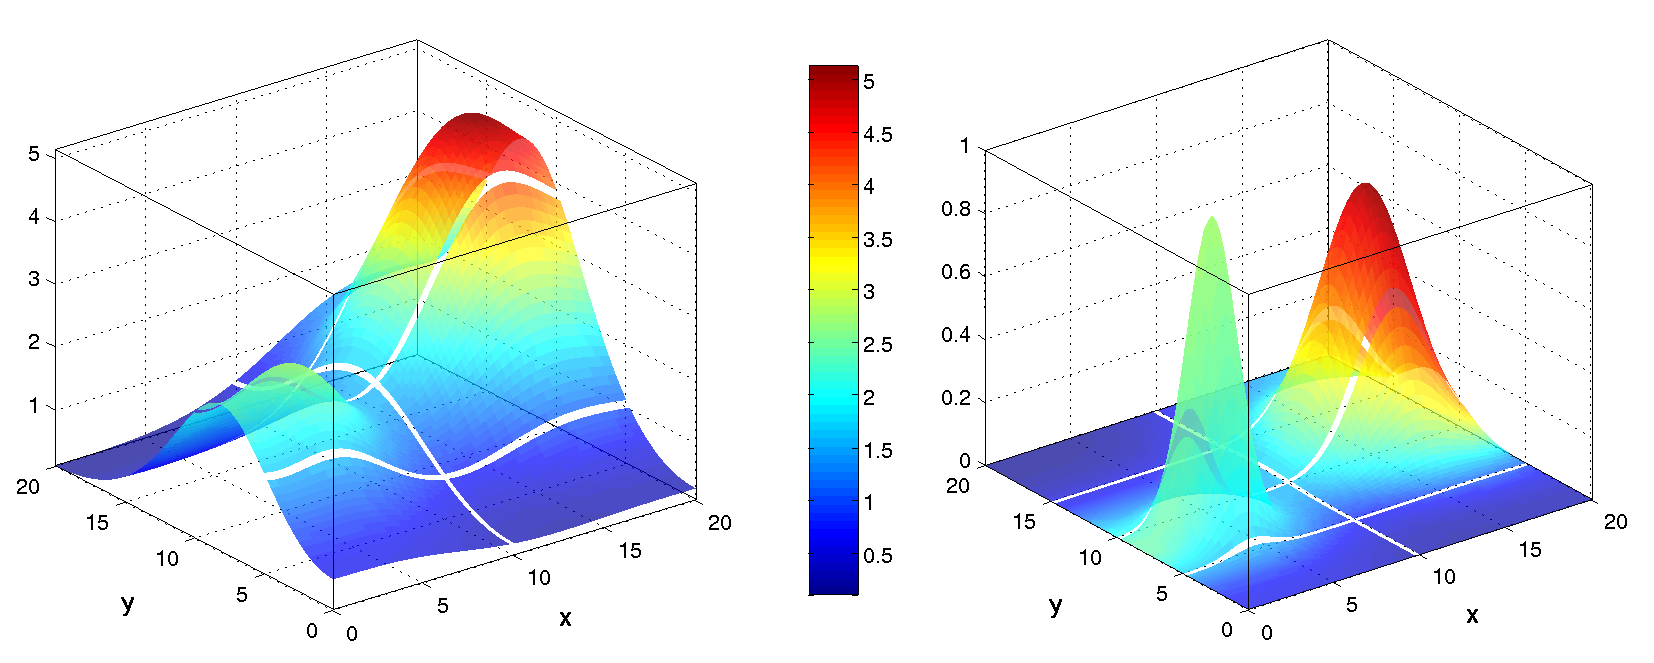
\epsfig{file=cvsadjkryx_p2D.eps,width=\textwidth}}}
  \caption{Results for the \id{cvsadjkryx\_p} example problem in 2D. 
    The gradient with respect to the source parameters is pictured on the left. 
    On the right, the gradient was color coded and superimposed over the nominal value 
    of the source parameters.}
  \label{f:cvsadjkryx_p2D}
\end{figure}
%%
%%
\begin{figure}
  {\centerline{\epsfig{file=cvsadjkryx_p3Dcf.eps,width=0.75\textwidth}}}
  \caption{Results for the \id{cvsadjkryx\_p} example problem in 3D.
  Nominal values of the source parameters.}\label{f:cvsadjkryx_p3D_a}
\end{figure}
%%
\begin{figure}
  {\centerline{\epsfig{file=cvsadjkryx_p3Dgrad.eps,width=0.75\textwidth}}}
  \caption{Results for the \id{cvsadjkryx\_p} example problem in 3D.
  Two isosurfaces of the gradient with respect to the source parameters.
  They correspond to values of $0.25$ (green) and $0.4$ (blue).}\label{f:cvsadjkryx_p3D_b}  
\end{figure}
%%
A sample output generated by \id{cvsadjkryx\_p} for a 2D calculation is shown below.

\includeOutput{cvsadjkryx\_p}{../examples_par/cvsadjkryx_p.out}


%===============================================================================
\section{Parallel tests}\label{s:ex_tests}
%===============================================================================


The most preeminent advantage of {\cvodes} over existing sensitivity solvers is
the possibility of solving very large-scale problems on massively parallel 
computers. To illustrate this point we present speedup results for the 
integration and forward sensitivity analysis for
an ODE system generated from the following 2-species diurnal
kinetics advection-diffusion PDE system in 2 space dimensions.
This work was reported in \cite{SeHi:03}.
The PDE takes the form:
\begin{equation*}
  \frac{dc_i}{dt} = K_h \frac{d^2c_i}{dx^2} + v \frac{dc_i}{dx} 
  + K_v \frac{d^2c_i}{dz^2}
  + R_i(c_1, c_2, t) \, , \quad \text{for } i=1,2 \, ,
\end{equation*}
where
\begin{equation*}
  \begin{split}
    R_1(c_1,c_2,t) &= -q_1 c_1 c_3 - q_2 c_1 c_2 + 2 q_3(t) c_3 + q_4(t) c_2 , \\
    R_2(c_1,c_2,t) &=  q_1 c_1 c_3 - q_2 c_1 c_2 - q_4(t) c_2 \, ,
  \end{split}
\end{equation*}
$K_h$, $K_v$, $v$, $q_1$, $q_2$, and $c_3$ are constants, and $q_3(t)$ and $q_4(t)$
vary diurnally.   
The problem is posed on the square
$0 \le x \le 20$, $30 \le z \le 50$   (all in km),
with homogeneous Neumann boundary conditions, and for time t in
$0 \le t \le 86400$ (1 day).
The PDE system is treated by central differences on a uniform
mesh, except for the advection term, which is treated with a biased
3-point difference formula.
The initial profiles are proportional to a simple polynomial in $x$
and a hyperbolic tangent function in $z$.

The solution with {\cvodes} is done with the BDF/GMRES method (i.e.
using the {\cvspgmr} linear solver) and the block-diagonal part of the 
Newton matrix as a left preconditioner. A copy of the block-diagonal
part of the Jacobian is saved and conditionally reused within the
preconditioner setup function.

The problem is solved by {\cvodes} on $P$ processors, treated as a 
rectangular process grid of size $p_x \times p_z$.
Each processor contains a subgrid of size $n = n_x \times n_z$ of the 
$(x,z)$ mesh.  Thus the actual mesh size is 
$N_x \times N_z = (p_x n_x) \times (p_z n_z)$,
and the ODE system size is $N = 2 N_x N_z$.
%%
Parallel performance tests were performed on ASCI Frost, a 68-node, 16-way SMP system
with POWER3 375 MHz processors and 16 GB of memory per node.
We present timing results for the integration of only the state equations
(column STATES), as well as for
the computation of forward sensitivities with respect to the diffusion coefficients
$K_h$ and $K_v$ using the staggered corrector method without and with 
error control on the sensitivity variables (columns STG and
STG\_FULL, respectively). 
Speedup results for a global problem size of
$N = 2 N_x N_y = 2 \cdot 1600 \cdot 400 = 1280000$ 
shown in Fig.~\ref{f:pvfktTest} and listed below.

\begin{center}
  \begin{tabular}{cccc}\hline
    $P$ &  STATES  &   STG   & STG\_FULL \\ \hline
    4  &  460.31  &  1414.53  & 2208.14  \\
    8  &  211.20  &   646.59  & 1064.94  \\
    16  &   97.16  &   320.78  &  417.95  \\
    32  &   42.78  &   137.51  &  210.84  \\
    64  &   19.50  &    63.34  &   83.24  \\
    128  &   13.78  &    42.71  &   55.17  \\
    256  &    9.87  &    31.33  &   47.95  \\ \hline
  \end{tabular}
\end{center}

%%
We note that there was not enough memory to solve the problem (even without
carrying sensitivities) on fewer processors.

The departure from the ideal line of slope $-1$ is explained by the 
interplay of several conflicting processes. On one hand, when increasing the 
number of processors, the preconditioner quality decreases, as it incorporates 
a smaller and smaller fraction of the Jacobian and the cost of inter-process 
communication increases. On the other hand, decreasing the number of processors
leads to an increase in the cost of the preconditioner setup phase and to a larger
local problem size which can lead to a point where a node starts memory paging to disk.
%%
%%
\begin{figure}
%%  {\centerline{\psfig{figure=pvfktTest.eps,width=0.5\textwidth}}}
  {\centerline{\epsfig{file=pvfktTest.eps,width=0.5\textwidth}}}
  \caption[Speedup results on a sensitivity problem]
  {Speedup results for the integration of the state equations only
    (solid line and column 'STATES'), staggered sensitivity analysis without
    error control on the sensitivity variables (dashed line and column 'STG'),
    and staggered sensitivity analysis with full error control (dotted line and
    column 'STG\_FULL')}
  \label{f:pvfktTest}
\end{figure}


%===============================================================
% References
\bibliographystyle{plain}
\bibliography{biblio}
%===============================================================
% Start appendices
\appendix
%% Forward sensitivity examples

\lstset{language=C}

\newpage
\section{Listing of cvsAdvDiff\_FSA\_non.c}\label{s:cvsAdvDiff_FSA_non_c}
\includeCode{../../examples/cvodes/serial/cvsAdvDiff_FSA_non.c}

\newpage
\section{Listing of cvsRoberts\_FSA\_dns.c}\label{s:cvsRoberts_FSA_dns_c}
\includeCode{../../examples/cvodes/serial/cvsRoberts_FSA_dns.c}

\newpage
\section{Listing of cvsDiurnal\_FSA\_kry\_p.c}\label{s:cvsDiurnal_FSA_kry_p_c}
\includeCode{../../examples/cvodes/parallel/cvsDiurnal_kry_p.c}

%% Adjoint sensitivity examples

\newpage
\section{listing of cvsRoberts\_ASAi\_dns.c}\label{s:cvsRoberts_ASAi_dns_c}
\includeCode{../../examples/cvodes/serial/cvsRoberts_ASAi_dns.c}

\newpage
\section{Listing of cvsAdvDiff\_ASAp\_non\_p.c}\label{s:cvsAdvDiff_ASAp_non_p_c}
\includeCode{../../examples/cvodes/parallel/cvsAdvDiff_ASAp_non_p.c}

\newpage
\section{Listing of cvsAtmDisp\_ASAi\_kry\_bbd\_p.c}\label{s:cvsAtmDisp_ASAi_kry_bbd_p_c}
\includeCode{../../examples/cvodes/parallel/cvsAtmDisp_ASAi_kry_bbd_p.c}

%===============================================================
\clearemptydoublepage
%\makeLLNLBackCover
%===============================================================
\end{document}